% !TeX root = constructions.tex

\chapter{How to Trisect an Angle (With a Little Help from a Friend)}\label{c.trisect}

It is well known that it is impossible to trisect an arbitrary angle using a compass and a straightedge. The reason is that trisection requires the construction of cube roots, but the compass and straightedge can only construct lengths that are expressions built from the four arithmetic operators and square roots.

Greek mathematicians discovered that if other instruments are allowed, angles can be trisected \cite{wiki:tri}. Section~\ref{s.neusis} presents a construction of Archimedes using a simple instrument called a \emph{neusis} \cite{wiki:neu}. Section~\ref{s.q} shows a more complex construction of Hippias using the \emph{quadratrix} \cite{wiki:quad}. As a bonus, Section~\ref{s.square} shows that the quadratrix can square a circle.

%%%%%%%%%%%%%%%%%%%%%%%%%%%%%%%%%%%%%%%%%%%%%%%%%%%%%%%%%%%%%

\section{Trisection using the neusis}\label{s.neusis}

In geometry textbooks, constructions are performed using a ``straightedge'' and a compass. The term straightedge is used instead of ``ruler'' because a straightedge has no marks on it. The only operation it can perform is to construct a straight line between two points, while a ruler can measure distances. To trisect an angle all we need is a straightedge with two marks that are a fixed distance apart, called a \emph{neusis}. We define the distance between the marks as $1$:
\begin{center}
\begin{tikzpicture}[scale=3.5]
\draw (-1,1.05) rectangle +(3.2,.1);
\draw[thick] (1.89,1.05) -- +(0,.1);
\draw[thick] (.73,1.05) -- +(0,.1);
\draw[<->] (.73,1.25) -- node[fill=white] {$1$} (1.89,1.25);
\end{tikzpicture}
\end{center}

Let $\alpha$ be an arbitrary angle $\angle ABE$ within a circle with center $B$ and radius $1$. The circle can be constructed by setting the compass to the distance between the marks on the neusis. Extend the radius $EB$ beyond the circle. Place an edge of the neusis on $A$ and move it until it intersects the extension of $EB$ at $D$ and the circle at $C$, using the marks so that the length of the line segment $CD$ is $1$. Draw the line $AD$:

\begin{center}
\begin{tikzpicture}[scale=2.5]
\coordinate (origin) at (0,0) node[below] {$B$} ;
\draw[name path=circle] (origin) circle [radius=1];
\draw (origin) node[above left,xshift=-4pt] {$\alpha$} -- (120:1) coordinate (a) node[below,xshift=-2pt] {$A$} ;
\draw (-1,0) -- (2.2,0);
\path[name path=ad] (a) -- (0,0 -| 2,0) coordinate (d) node[below] {$D$} ;
\path[name intersections={of=circle and ad,by={c,a1}}];
\fill (origin) circle [radius=.5pt];
\fill (a) circle [radius=.5pt];
\fill (c) circle [radius=.5pt] node [below,xshift=-4pt] {$C$};
\fill (d) circle [radius=.5pt];
\fill (-1,0) circle [radius=.5pt] node [left] {$E$};
\begin{scope}[rotate=-19,yshift=-11.25pt]
\draw (-1,1.05) rectangle +(3.2,.1);
\draw[thick] (1.89,1.05) -- +(0,.1);
\draw[thick] (.76,1.05) -- +(0,.1);
\draw[<->] (.73,1.25) -- node[fill=white] {$1$} (1.89,1.25);
\end{scope}
\end{tikzpicture}
\end{center}

\newpage

Draw line $BC$ and label the angles and line segments as shown:

\begin{center}
\begin{tikzpicture}[scale=2.5]
\coordinate (origin) at (0,0) node[below] {$B$} ;
\draw[name path=circle] (origin) circle [radius=1];
\draw (origin) node[above left,xshift=-4pt] {$\alpha$} node[above,xshift=4pt,yshift=2pt] {$\delta$} node[above right,xshift=44pt,yshift=-2pt] {$\beta$} -- node[fill=white] {$1$} (120:1) coordinate (a) node[above left] {$A$} ;
\draw (-1,0) -- (2.2,0);
\draw[name path=ad] (a) node[below right,xshift=8pt,yshift=-6pt] {$\gamma$} -- (0,0 -| 2,0) coordinate (d) node[left,xshift=-50pt,yshift=7pt] {$\beta$} node[above right] {$D$} ;
\path[name intersections={of=circle and ad,by={c,a1}}];
\draw (origin) -- node[fill=white] {$1$}(c) node[above right] {$C$} node[left,xshift=-12pt] {$\gamma$} node[below,xshift=-2pt,yshift=-4pt] {$\epsilon$};
\fill (origin) circle [radius=.5pt];
\fill (a) circle [radius=.5pt];
\fill (d) circle [radius=.5pt];
\fill (c) circle [radius=.5pt];
\fill (-1,0) circle [radius=.5pt];
\path (c) -- node[fill=white] {$1$} (d);
%\begin{scope}[rotate=-20]
%\draw (-1,1.05) rectangle +(3.2,.1);
%\draw[thick] (1.89,1.05) -- +(0,.1);
%\draw[thick] (.73,1.05) -- +(0,.1);
%\draw[<->] (.73,1.25) -- node[fill=white] {$1$} (1.89,1.25);
%\end{scope}
\end{tikzpicture}
\end{center}

Both $\triangle ABC$ and $\triangle BCD$ are isoceles: $AB=BC$ since both are radii and $BC=CD$ by construction using the neusis. A computation (using the facts that the angles of a triangle and supplemenary angles add up to $180$ radians) shows that $\beta$ trisects $\alpha$:
\erh{1pt}
\begin{equationarray*}{rcl}
\epsilon &=& \pi - 2\beta\\
\gamma &=& \pi - \epsilon = 2\beta\\
\delta &=& \pi - 2\gamma = \pi - 4\beta\\
\alpha &=& \pi - \delta - \beta\\
&=& 4\beta -\beta\\
&=& 3\beta\,.
\end{equationarray*}

\vspace{-2ex}

%%%%%%%%%%%%%%%%%%%%%%%%%%%%%%%%%%%%%%%%%%%%%%%%%%%%%%%%%%%%%

\section{Trisection using the quadratrix}\label{s.q}

The following diagram shows a \emph{quadratrix compass}: two (unmarked) straightedges connected by a joint that constrains them to move together. One straightedge moves parallel to the $x$-axis from $DC$ to $AB$, while the second straightedge is allowed to rotate around the origin at $A$ until it lies horizontally along $AB$. The curve traced by the joint of the two straightedges is called the \emph{quadratrix curve} or simply the \emph{quadratrix}.

\begin{center}
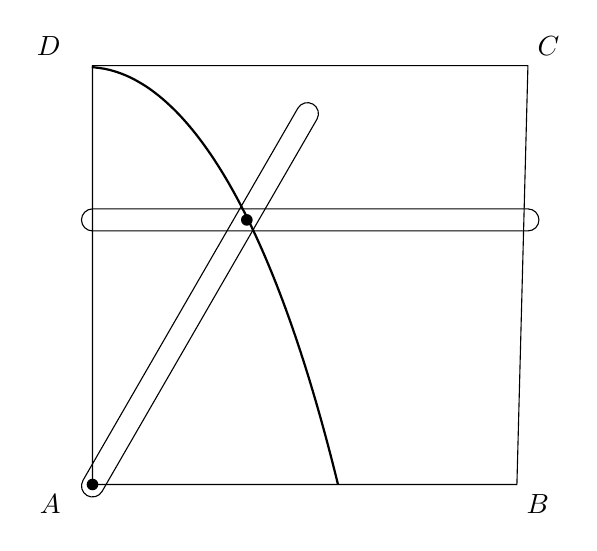
\begin{tikzpicture}[scale=.7,domain=.03:1.555,samples=100]
\draw (.1,.2) node[below left,xshift=-8pt] {$A$} -- (7.8,.2) node[below right] {$B$} -- (8,7.8) node[above right] {$C$} -- (.1,7.8) node[above left,xshift=-8pt] {$D$} -- cycle;
%\draw (.1,7.8) -- (.1,.2) -- (8,.1) -- (8,7.8);
\draw[rounded corners,rotate=60] (0,-.2) rectangle (8.2,.2);
\draw[rounded corners] (-.1,4.8) rectangle (8.2,5.2);
\fill (2.9,5) circle [radius=3pt];
\fill (.1,.2) circle [radius=3pt];
\draw[thick] plot (4.6*.637*\x,{12.2*.637*\x*cot(\x r)});
\end{tikzpicture}
\end{center}

\vspace{-2ex}

As the horizontal straightedge is moved down at a constant velocity, the other straightedge is constrained to move at a constant angular velocity. In fact, that is the definition of the quadratrix curve. As the $y$-coordinate of the horizontal straightedge decreases from $1$ to $0$, the angle of the other straightedge relative to the $x$-axis decreases from $90^\circ$ to $0^\circ$. The following diagram shows how this can be used to trisect an arbitrary angle $\alpha$:

\vspace{-2ex}

\begin{center}
\begin{tikzpicture}[scale=.7,domain=.03:1.562,samples=100]
\draw (.1,7.8) coordinate (start) node[above left] {$D$} node[below right,xshift=32pt] {$\theta$} -- (.1,.2) node[below left] {$A$} -- (8,.1) node[below right] {$B$} -- (8,7.8) node[above right] {$C$} -- cycle;
\draw[name path=curve,thick] plot (4.6*.637*\x,{12.2*.637*\x*cot(\x r)});
% To ensure intersection at node D, path should extend to the upper left of D
\coordinate (twenty-a) at ($(start)+(-35:9)$);
\path[name path=twenty] ($(start)!-.1!(twenty-a)$) -- (twenty-a);
\path[name path=sixty] (start) -- +(-50:9);
\path[name path=xaxis] (.1,.2) -- (8,.1);
\path[name intersections={of=twenty and curve,by={x1,tri}}];
\draw (start) -- (tri);
\fill (tri) circle [radius=2pt] node[right] {$P_2$};
\path[name intersections={of=sixty and curve,by={x2,angle}}];
\fill (angle) circle [radius=2pt] node[right] {$P_1$};
\draw (start) -- (angle);
\path[name intersections={of=xaxis and curve,by=x}];
\fill (x) circle [radius=2pt];
%\path (.1,.2) -- node[below] {$2/\pi$} (x);
\draw[dashed] (tri) -- (tri -| .1,.2) coordinate (t3);
\fill (t3) circle [radius=2pt] node[left] {$F$};
\draw[dashed] (angle) -- (angle -| .1,.2) coordinate (t);
\fill (t) circle [radius=2pt] node[left] {$E$};
\draw[<->] (-1.2,7.8) -- node[fill=white] {$t/3$} (-1.2,7.8 |- t3);
\draw[<->] (-.6,7.8) -- node[fill=white] {$t$} (-.6,7.8 |- t);
\draw[<->] (-.6,7.8 |- t) -- node[fill=white] {$1-t$} (-.6,.2);
\draw (3.5,7.8) arc[start angle=0,delta angle=-49,radius=3.5];
\draw (1,7.8) arc[start angle=0,delta angle=-32,radius=1];
\node at (3.3,6) {$\alpha$}; 
\end{tikzpicture}
\end{center}

\vspace{-2ex}

$P_1$ is the intersection of the line defining the angle $\alpha$ with the quadratrix. This point has $y$-coordinate $1-t$, where $t$ is the distance that the horizontal straightedge has moved from its initial position $DC$. Now trisect the \emph{line segment} $DE$ to obtain point $F$. (It is easy to trisect a line segment using Thales theorem.) Let $P_2$ be the intersection of a line from $F$ parallel to $DC$ and the quadratrix. By the equality of the velocities, we have:

\vspace{-2ex}

\erh{0pt}
\begin{equationarray*}{rcl}
\frac{\theta}{\alpha} &=& \frac{t/3}{t}\\
&&\\
\theta &=& \alpha/3\,.
\end{equationarray*}

\vspace{-3ex}

%%%%%%%%%%%%%%%%%%%%%%%%%%%%%%%%%%%%%%%%%%%%%%%%%%%%%%%%%%%%%

\section{Squaring the circle using the quadratrix}\label{s.square}

\begin{center}
\begin{tikzpicture}[scale=.7,domain=.01:1.57,samples=100]
\draw (0,0) node[below left] {$A$} node [above right,xshift=10pt] {$\theta$} -- (8,0) node[below right] {$B$} -- (8,8) node[above right] {$C$} -- (0,8) node[above left] {$D$} -- cycle;
\draw[name path=horiz] (0,5) -- (8,5);
\draw[name path=slant] (0,0) -- (61:8);
\path[name intersections={of=horiz and slant,by=joint}];
\draw[dashed] (joint) -- node[right] {$y$} (joint |- 0,0) coordinate (f);
\path (0,0) -- node[below] {$x$} (0,0 -| joint) node[below] {$F$};
\path (0,5) node[left] {$E$} -- node[left] {$t$} (0,8);
\path (0,0) -- node[left] {$1-t$} (0,5);
\fill (joint) circle [radius=2pt] node[above right,xshift=4pt] {$P$};
\fill (f) circle [radius=2pt];
\fill (0,5) circle [radius=2pt];
\fill (4.28,0) circle [radius=2pt] node[below] {$G$};
\draw[name path=curve,thick] plot (4.3*.637*\x,{12.5*.637*\x*cot(\x r)});
\end{tikzpicture}
\end{center}

Suppose that the horizontal straightedge has moved $t$ down the $y$-axis to point $E$ and the rotating straightedge forms an angle of $\theta$ with the $x$-axis. $P$ is the intersection of the quadratrix with the horizontal straightedge, and $F$ is the projection of $P$ on the $x$-axis. What are the coordinates of quadratrix at $P$? Clearly, $y=PF=EA=1-t$. On the quadratrix, $\theta$ decreases at the same rate that $t$ increases:
\erh{0pt}
\begin{equationarray*}{rcl}
\frac{1-t}{1} &=& \frac{\theta}{\pi/2}\\
&&\\
\theta &=&\frac{\pi}{2}(1-t)\,.
\end{equationarray*}
Check if this makes sense: when $t=0$, $\theta=\pi/2$ and when $t=1$, $\theta=0$.

The $x$-coordinate of $P$ follows from trigonometry:
\[
\tan \theta = \frac{y}{x}\,.
\]
which gives:
\[
x = \frac{y}{\tan\theta}=y\cot\theta=y\cot \frac{\pi}{2}(1-t)=y\cot \frac{\pi}{2}y\,.
\]
We usually express a function as $y=f(x)$ but it can also be expressed as $x=f(y)$. Let us compute the $x$-coordinate of the point $G$, the intersection of the quadratrix with the $x$-axis. We can't simply plug in $y=0$ because $\cot 0$ is not defined, but we might get lucky by computing the limit of $x$ as $y$ goes to $0$:
\[
x = y\cot \frac{\pi}{2}y = \frac{2}{\pi}\cdot \frac{\pi}{2}y\cot \frac{\pi}{2}y\,.
\]
For convenience, perform a change of variable $z=\disfrac{\pi}{2}y$ and compute the limit:
\[
\lim_{z\rightarrow 0} z\cot z = \lim_{z\rightarrow 0} \frac{z\cos z}{\sin z} = \lim_{z\rightarrow 0} \frac{\cos z}{\disfrac{\sin z}{z}} = \frac{\cos 0}{1} = 1\,,
\]
using the well-known fact that $\displaystyle\lim_{z\rightarrow 0} \frac{\sin z}{z}=1$.
Therefore, as $y\rightarrow 0$:
\[
x \rightarrow \frac{2}{\pi}\cdot \lim_{y\rightarrow 0}\frac{\pi}{2}y\cot \frac{\pi}{2}y = \frac{2}{\pi}\cdot 1 = \frac{2}{\pi}\,.
\]
Using the quadratrix we have constructed a line segment $AG$ whose length is $x=\displaystyle\frac{2}{\pi}$. With an ordinary straightedge and compass it is easy to construct a line segment of length $\sqrt{\disfrac{2}{x}}=\sqrt{\pi}$ and then construct a square whose area is $\pi$.


